% !TEX program = pdflatex
%Numerical Experiment_2
\documentclass[10pt,a4paper]{article}
\usepackage[UTF8]{ctex}
\usepackage{bm}
\usepackage{amsmath}
\usepackage{amssymb}
\usepackage{graphicx}
%\usepackage{geometry}
%\geometry{a4paper,left=.3cm,right=.3cm,top=1cm,bottom=1.5cm}
\usepackage{float}
\usepackage{multirow}
\usepackage{listings}
\usepackage[framed,numbered,autolinebreaks,useliterate]{mcode}
\usepackage{textcomp}
\usepackage{setspace}
\title{数值试验二报告}
\author{陈稼霖 \and 45875852}
\date{2019.4.23}
\begin{document}
\maketitle
1.(1)对函数$f(x)=\frac{1}{1+25x^2}$,在区间$[-1,1]$用拉格朗日插值法进行插值,取不同的插值多项式的阶数,观察龙格现象.\\
解:在$-1$与$1$之间取等距节点
\[
x_i=-1+\frac{2i}{n},~~i=0,1,2,\cdots,n
\]
分别做阶数$n=2,4,6,8$的拉格朗日插值多项式,作图如下. 可见,在接近端点$-1$与$1$的地方插值结果就会出现震荡,且$n$越大,这种振荡越剧烈.
\begin{figure}[H]
\centering
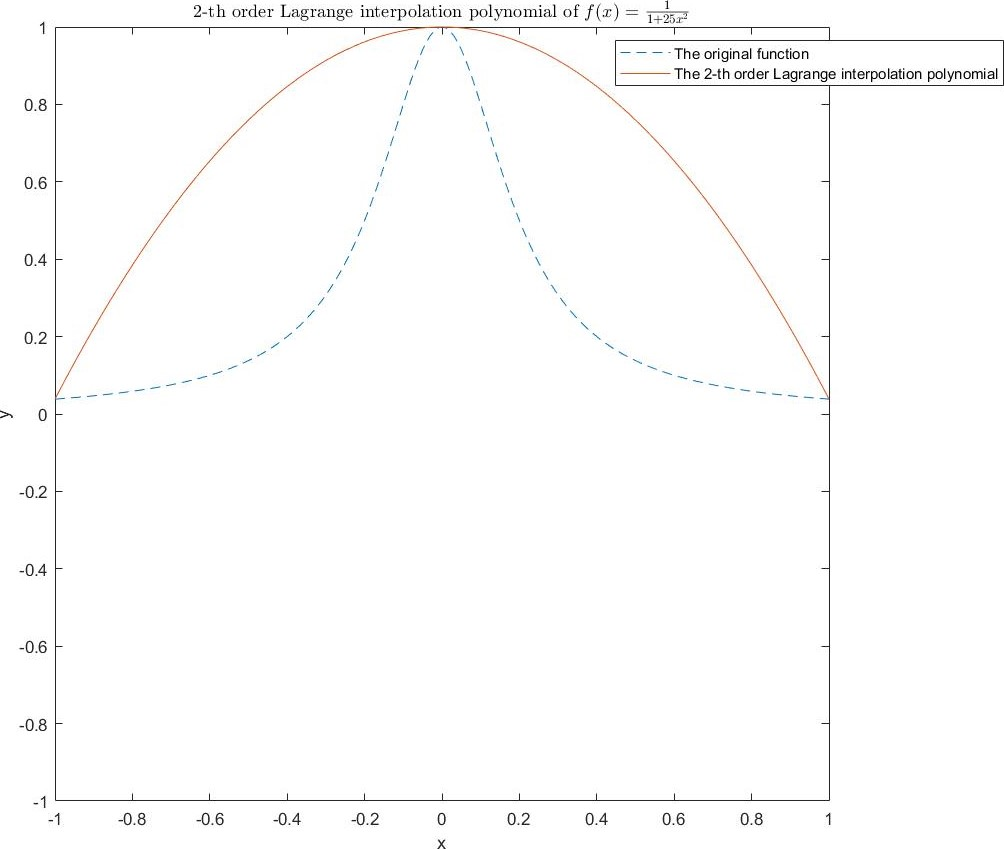
\includegraphics[scale=.4]{1_1_1.jpg}
\caption{2阶拉格朗日插值多项式和原函数}
\end{figure}
\newpage
\begin{figure}[H]
\centering
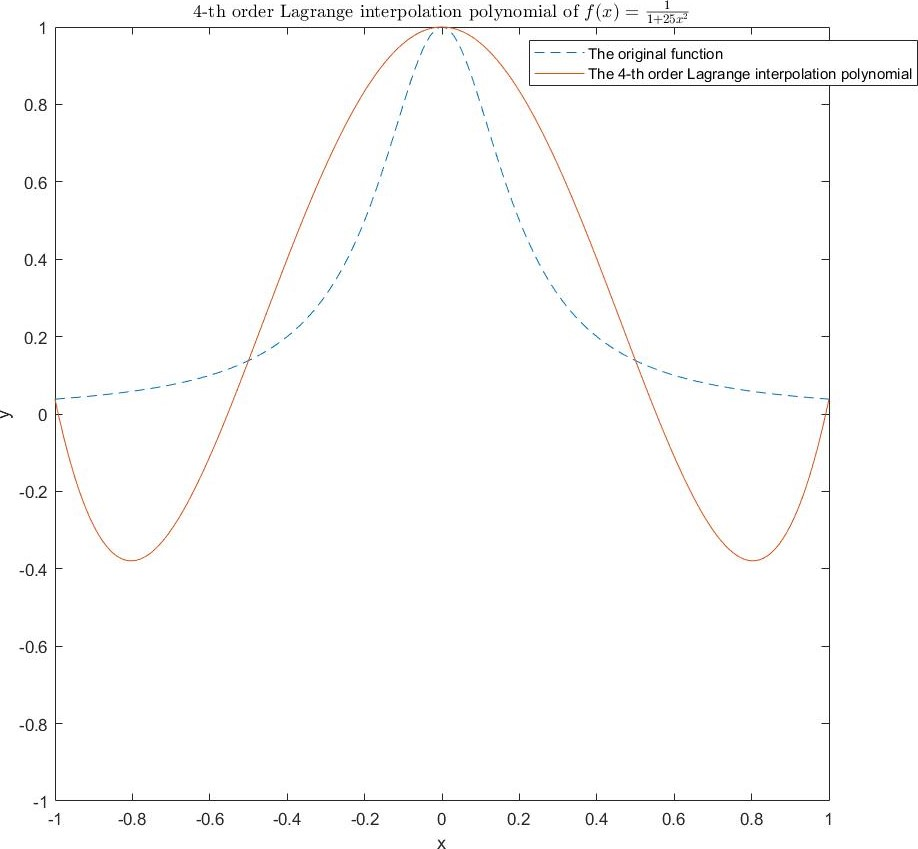
\includegraphics[scale=.4]{1_1_2.jpg}
\caption{4阶拉格朗日插值多项式和原函数}
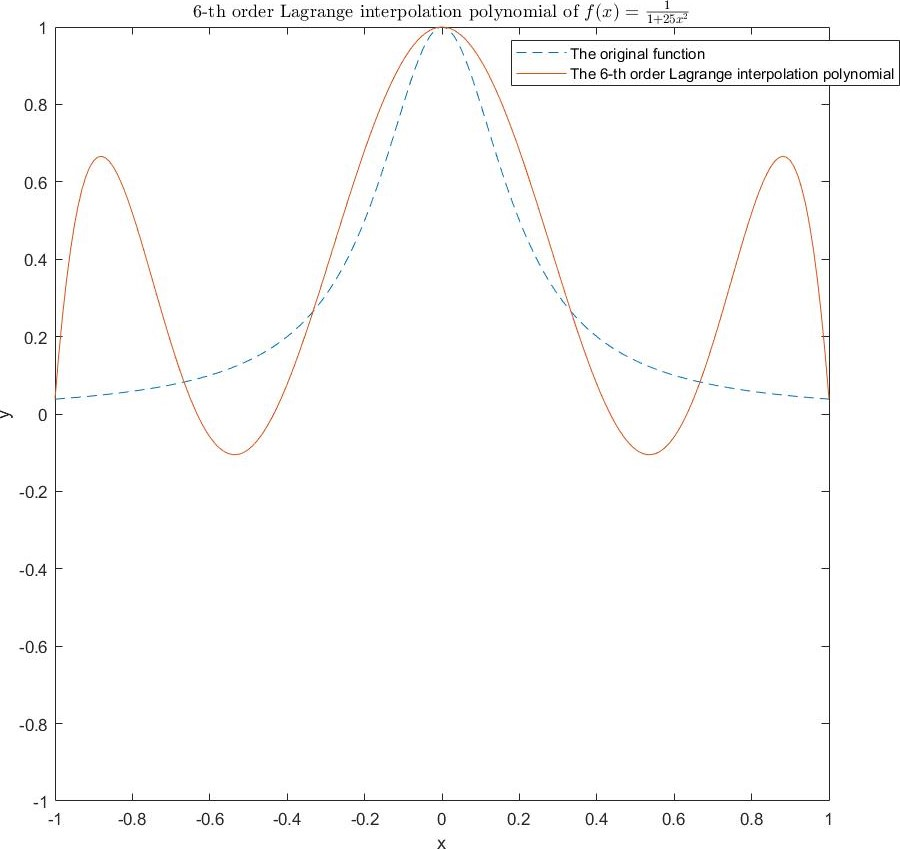
\includegraphics[scale=.4]{1_1_3.jpg}
\caption{6阶拉格朗日插值多项式和原函数}
\end{figure}
\newpage
\begin{figure}[H]
\centering
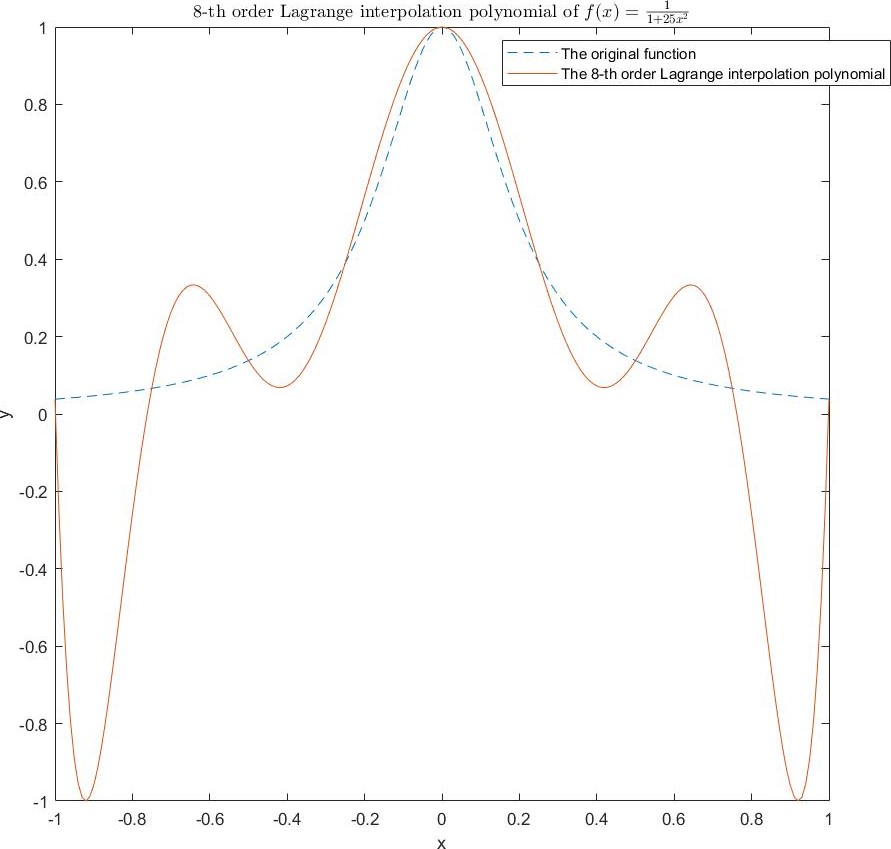
\includegraphics[scale=.4]{1_1_4.jpg}
\caption{8阶拉格朗日插值多项式和原函数}
\end{figure}

(2)求$f(x)$在$[-1,1]$上的最佳平方逼近多项式$P_4(x)=a+bx^2+cx^4$.\\
解:记
\[
I=\int_{-1}^1[f(x)-P_4(x)]^2dx\triangleq\int_{-1}^1[\frac{1}{1+25x^2}-(a+bx^2+cx^4)]^2dx
\]
最佳平方逼近要求
\begin{gather*}
\left\{\begin{array}{ll}
\frac{\partial I}{\partial a}=&-2\int_{-1}^1[\frac{1}{1+25x^2}-(a+bx^2+cx^4)]dx\\
&=-2[\frac{2}{5}\arctan5-2a-\frac{2}{3}b-\frac{2}{5}c]=0\\
\frac{\partial I}{\partial b}=&-2\int_{-1}^1x^2[\frac{1}{1+25x^2}-(a+bx^2+cx^4)]dx\\
&=-2(\frac{2}{25}-\frac{2}{125}\arctan5-\frac{2}{3}a-\frac{2}{5}b-\frac{2}{7}c)=0\\
\frac{\partial I}{\partial b}=&-2\int_{-1}^1x^4[\frac{1}{1+25x^2}-(a+bx^2+cx^4)]dx\\
&=-2[\frac{44}{1875}+\frac{2}{3125}\arctan5-\frac{2}{5}a-\frac{2}{7}b-\frac{2}{9}c]=0\\
\end{array}\right.\\
\Longrightarrow\left\{\begin{array}{l}
a=\frac{3(-1610+2797\arctan5)}{10000}\\
b=-\frac{21(-180+211\arctan5)}{1000}\\
c=\frac{21(-370+399\arctan5)}{2000}\\
\end{array}\right.
\end{gather*}
故$f(x)$在$[-1,1]$上的最佳平方逼近多项式为
\footnotesize\[
P_4(x)=\frac{3(-1610+2797\arctan5)}{10000}-\frac{21(-180+211\arctan5)}{1000}x^2+\frac{21(-370+399\arctan5)}{2000}x^4
\]\normalsize
(3)用复合Simpson公式计算$(\int_{-1}^1[f(x)-P_4(x)]^2dx)^{\frac{1}{2}}$,即用$P_4(x)$逼近$f(x)$的均匀方差.\\
解:将区间$[-1,1]$做$200$等分,即取节点
\[
x_i=-1+\frac{i}{100},~~i=0,1,2,\cdots,200
\]
用$P_4(x)$逼近$f(x)$的均匀方差为
\small\begin{align*}
(\int_{-1}^1[f(x)-P_4(x)]^2dx)^{\frac{1}{2}}\approx&\{\sum_{i=0}^{199}\frac{2}{6\times200}[(f(x_i)-P_4(x_i))^2+4(f(x_{i+\frac{1}{2}})-P_4(x_{i+\frac{1}{2}}))^2\\
&+(f(x_{i+1})-P_4(x_{i+1}))^2]\}^{\frac{1}{2}}\\
=&0.1835
\end{align*}\normalsize

2. \textbf{世界人口数据拟合问题}据统计六十年代世界人口数据如下(单位:亿)\\
\begin{table}[h]
\begin{tabular}{|c|c|c|c|c|c|c|c|c|c|}
\hline
年  & 1960  & 1961  & 1962  & 1963  & 1964  & 1965  & 1966  & 1967  & 1968  \\ \hline
人口 & 29.72 & 30.61 & 31.51 & 32.13 & 32.34 & 32.85 & 33.56 & 34.20 & 34.83 \\ \hline
\end{tabular}
\end{table}
根据表中数据,预测2018年($76$亿)、2019年时的世界人口。

\noindent\textbf{问题分析与数学模型}\\
\indent设人口总数为$N(t)$,根据人口理论的马尔萨斯模型,采用指数函数
\begin{equation}
\label{Malthus}
N(t)=e^{a+bt}
\end{equation}
对数据进行拟合。为了计算方便,将上式两边同时取对数,得$\ln N=a+bt$,令
\[
y=\ln N\text{ 或 }N=e^y
\]
变换后的拟合函数为
\[
y(t)=a+bt
\]
有人口取对数($y=\ln N$)计算,得下表
\begin{table}[h]
\footnotesize
\begin{tabular}{|c|c|c|c|c|c|c|c|c|c|}
\hline
t & 1960   & 1961   & 1962   & 1963   & 1964   & 1965   & 1966   & 1967   & 1968   \\ \hline
y & 3.3918 & 3.4213 & 3.4503 & 3.4698 & 3.4763 & 3.4920 & 3.5133 & 3.5322 & 3.5505 \\ \hline
\end{tabular}
\end{table}
\\根据表中数据及等式$a+bt_k=y_k~~(k=1,2,\cdots,9)$可列出关于两个未知数$a$、$b$的9个方程的超定方程组(方程数多于未知数个数的方程组)
\[
a+t_jb=y_j
\]
可用最小二乘法求解。

\noindent\textbf{算法与数学模型求解}\\
算法如下:\\
第一步:输入入口数据,并计算所有人口数据的对数值;\\
第二步:建立超定方程组的系数矩阵,并计算对应的正规方程组的系数矩阵和右端向量;\\
第三步:求解超定方程组并输出结果:$a$,$b$;\\
第四步:利用数据结果构造指数函数计算$2018$、$2019$年人口近似值,结束。

\noindent超定方程组的系数矩阵为
\[
A=\left[\begin{array}{cc}
1 & 1960 \\
1 & 1961 \\
1 & 1962 \\
1 & 1963 \\
1 & 1964 \\
1 & 1965 \\
1 & 1966 \\
1 & 1967 \\
1 & 1968 \\
\end{array}\right]
\]
超定方程组的右端向量为
\[
y=\left[\begin{array}{c}
3.3918 \\
3.4213 \\
3.4503 \\
3.4698 \\
3.4763 \\
3.4920 \\
3.4831 \\
3.5322 \\
3.5505 \\
\end{array}\right]
\]
正规方程组的系数矩阵为
\[
A^TA=\left[\begin{array}{cc}
9 & 17676 \\
17676 & 34715724 \\
\end{array}\right]
\]
正规方程组的右端矢量为
\[
A^Ty=\left[\begin{array}{c}
31.2673 \\
61410.0086 \\
\end{array}\right]
\]
求解$A^TA\left[\begin{array}{l}a\\b\end{array}\right]=A^Ty$得
\[
\left[\begin{array}{l}a\\b\end{array}\right]=\left[\begin{array}{c}-31.0613 \\0.0176 \\\end{array}\right]
\]
将$a$、$b$代入式(\ref{Malthus}),再分别代入$t=2018$和$t=2019$得到2018年和2019年时的世界人口近似值(亿)
\begin{align*}
N(2018)=&e^{-31.0613+0.0176\times2018}=83.4035\\
N(2019)=&e^{-31.0613+0.0176\times2019}=84.8831
\end{align*}
\begin{figure}[H]
\centering
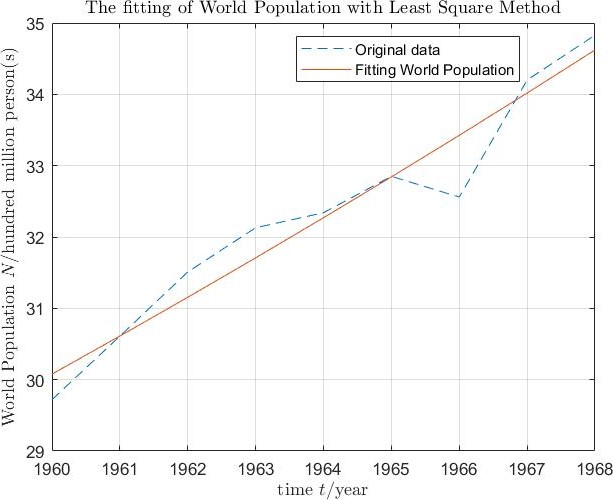
\includegraphics[scale=.5]{2.jpg}
\caption{世界人口及其拟合曲线}
\end{figure}

3. \textbf{SARS的传播及预防问题}\\
\indent非典的爆发和蔓延给我国的经济发展和人民生活带来了很大的影响,下标给出了北京市当年4月份到6月份的疫情数据,通过拟合确诊的累计病人曲线,若延后5天采取严格的预防措施,对疫情的传播所生成的影响作出估计.
\begin{table}[h]
\begin{tabular}{|c|c|c|c|c|}
\hline
日期    & 已确诊病例累计 & 现有疑似病例 & 死亡累计 & 治愈出院累计 \\ \hline
4月20日 & 297     & 402    & 18   & 33     \\ \hline
4月30日 & 1584    & 1408   & 75   & 90     \\ \hline
5月1日  & 1640    & 1415   & 82   & 100    \\ \hline
5月10日 & 1988    & 1397   & 116  & 175    \\ \hline
5月20日 & 2189    & 1225   & 150  & 395    \\ \hline
5月30日 & 2309    & 706    & 176  & 1006   \\ \hline
6月1日  & 2319    & 739    & 181  & 1124   \\ \hline
6月10日 & 2394    & 351    & 184  & 1747   \\ \hline
6月20日 & 2439    & 3      & 191  & 2189   \\ \hline
\end{tabular}
\end{table}
\newpage
取拟合曲线的拟合函数为如下非线性函数
\[
\frac{1}{y}=a+\frac{b}{x}
\]
试确定拟合函数中的参数:$a$,$b$,并推测五天后累计病人数量。

算法如下:\\
第一步:输入时间$t$(天)和累计确诊病例数$N$,并分别计算其倒数,
\begin{table}[h]
\scriptsize
\begin{tabular}{|c|c|c|c|}
\hline
时间$t$(天) & 时间的倒数$\frac{1}{t}$(天$^{-1}$) & 累计确诊病例数$N$(人) & 累计确诊病例数$\frac{1}{N}$(人$^{-1}$) \\ \hline
1        & 1                            & 297           & $\frac{1}{297}$                \\ \hline
11       & $\frac{1}{11}$               & 1584          & $\frac{1}{1584}$               \\ \hline
22       & $\frac{1}{22}$               & 1640          & $\frac{1}{1640}$               \\ \hline
31       & $\frac{1}{31}$               & 1988          & $\frac{1}{1988}$               \\ \hline
41       & $\frac{1}{41}$               & 2189          & $\frac{1}{2189}$               \\ \hline
51       & $\frac{1}{51}$               & 2309          & $\frac{1}{2309}$               \\ \hline
53       & $\frac{1}{53}$               & 2319          & $\frac{1}{2319}$               \\ \hline
62       & $\frac{1}{62}$               & 2396          & $\frac{1}{2394}$               \\ \hline
72       & $\frac{1}{72}$               & 2439          & $\frac{1}{2439}$               \\ \hline
\end{tabular}
\end{table}
\\第二步:建立超定方程组的系数矩阵和右端向量
\[
A=\left[\begin{array}{cc}
1 & \frac{1}{1} \\
1 & \frac{1}{11} \\
1 & \frac{1}{22} \\
1 & \frac{1}{31} \\
1 & \frac{1}{41} \\
1 & \frac{1}{51} \\
1 & \frac{1}{53} \\
1 & \frac{1}{62} \\
1 & \frac{1}{72} \\
\end{array}\right],~~b=\left[\begin{array}{c}
\frac{1}{297} \\
\frac{1}{1584} \\
\frac{1}{1640} \\
\frac{1}{1988} \\
\frac{1}{2189} \\
\frac{1}{2309} \\
\frac{1}{2319} \\
\frac{1}{2394} \\
\frac{1}{2439} \\
\end{array}\right]
\]
并计算对应的正规方程组的系数矩阵和右端向量
\[
A^TA=\left[\begin{array}{cc}
9 & 1.2615 \\
1.2615 & 1.0132 \\
\end{array}\right],~~A^Tb=\left[\begin{array}{c}
0.0073 \\
0.0035 \\
\end{array}\right]
\]
第三步:求解$A^TA=A^Tb$并输出结果
\[
\left[\begin{array}{l}a\\b\end{array}\right]=\left[\begin{array}{l}0.0004\\0.0030\end{array}\right]
\]
第四步:利用数据结果构造非线性函数
\[
\frac{1}{N}=0.0004+\frac{0.0030}{t}
\]
并计算五天后累计病人数量
\[
N(77)=\frac{1}{0.0004+\frac{0.0030}{77}}=2337
\]
\begin{figure}[H]
\centering
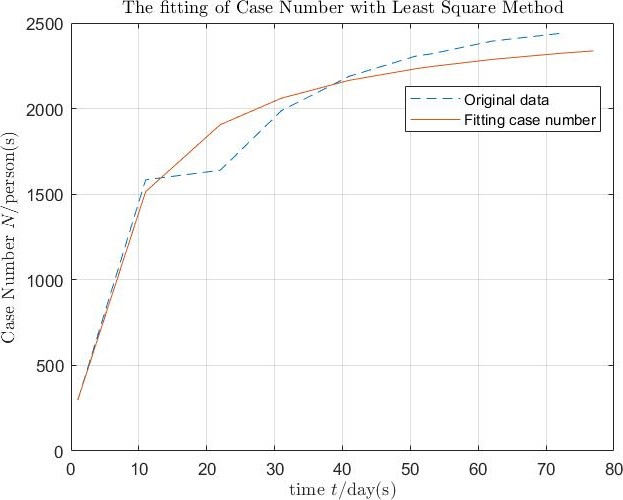
\includegraphics[scale=.5]{3.jpg}
\caption{累计确诊病例数及其拟合曲线}
\end{figure}

\textbf{MATLAB/Mathematica代码}\\
1.(1)拉格朗日插值法Matlab代码
\begin{lstlisting}
close,clear,clc;
for n = 2:2:8% the number of the nodes
    x = 2 / n * (0:n)' - 1;% the nodes
    L = @(t)L_n(t,x);% lagrange interpolation polynomial corresponding to the nodes
    t = -1:0.01:1;
    %subplot(2,2,floor((n / 2 - 1) / 2) + 2 * mod(n / 2 - 1,2) + 1);
    figure(n / 2);
    plot(t,f(t),'--');
    hold on;
    plot(t,L(t));
    axis square
    ylim([-1,1]);
    title([num2str(n),'-th order Lagrange interpolation polynomial of $f(x)=\frac{1}{1+25x^2}$'],'Interpreter','LaTeX')
    xlabel('x');
    ylabel('y');
    legend('The original function',['The ',num2str(n),'-th order Lagrange interpolation polynomial']);
end

function y = f(x)
y = 1 ./ (1 + 25 * x.^2);
end
function y = L_n(t,x)
n = size(x,1) - 1;
y = 0;
for i = 0:n
    l_i = f(x(i + 1));
    for j = 0:n
        if j ~= i
            l_i = l_i .* (t - x(j + 1)) / (x(i + 1) - x(j + 1));
        end
    end
    y = y + l_i;
end
end
\end{lstlisting}
(2)解线性代数方程组Mathematica代码\\
\begin{doublespace}
\noindent\(\pmb{m=\{\{2,2/3,2/5\},\{2/3,2/5,2/7\},\{2/5,2/7,2/9\}\}}\)
\end{doublespace}

\begin{doublespace}
\noindent\(\left\{\left\{2,\frac{2}{3},\frac{2}{5}\right\},\left\{\frac{2}{3},\frac{2}{5},\frac{2}{7}\right\},\left\{\frac{2}{5},\frac{2}{7},\frac{2}{9}\right\}\right\}\)
\end{doublespace}

\begin{doublespace}
\noindent\(\pmb{n=\{\text{Integrate}[1/(1+25 x{}^{\wedge}2),\{x,-1,1\}],}\\
\pmb{\text{Integrate}[x{}^{\wedge}2/(1+25 x{}^{\wedge}2),\{x,-1,1\}],}\\
\pmb{\text{Integrate}[x{}^{\wedge}4/(1+25 x{}^{\wedge}2),\{x,-1,1\}]\}}\)
\end{doublespace}

\begin{doublespace}
\noindent\(\left\{\frac{2 \text{ArcTan}[5]}{5},-\frac{2}{125} (-5+\text{ArcTan}[5]),\frac{220+6 \text{ArcTan}[5]}{9375}\right\}\)
\end{doublespace}

\begin{doublespace}
\noindent\(\pmb{\text{Solve}[m.\{a,b,c\}==n,\{a,b,c\}]}\)
\end{doublespace}

\begin{doublespace}
\noindent\(\left\{\left\{a\to \frac{3 (-1610+2797 \text{ArcTan}[5])}{10000},b\to -\frac{21 (-180+211 \text{ArcTan}[5])}{1000},c\to \frac{21 (-370+399
\text{ArcTan}[5])}{2000}\right\}\right\}\)
\end{doublespace}

\noindent(3)复合Simpson公式计算积分Matlab代码
\begin{lstlisting}
close,clear,clc;
x = -1:0.01:1;
plot(x,f(x),'--');
hold on;
plot(x,P_4(x));
axis square;
delta = @(x)(f(x) - P_4(x)).^2;
n = 200;
I = 0;
for i = 0:(n - 1)
    I = I + 2 / (6 * n) * (delta(-1 + 2 * i / n) + 4 * delta(-1 + 2 * (i + 1 / 2) / n) + delta(-1 + 2 * (i + 1) / n));
end
I = sqrt(I);
function y = f(x)
    y = 1 ./ (1 + 25 * x.^2);
end
function y = P_4(x)
    y = 3 * (-1610 + 2797 * atan(5)) / 10000 - 21 * (-180 + 211 * atan(5)) / 1000 * x.^2 + 21 * (-370 + 399 * atan(5)) / 2000 * x.^4;
end
\end{lstlisting}
2. 最小二乘法拟合世界人口Matlab代码
\begin{lstlisting}
close,clear,clc;
t = (1960:1968)';% time (year)
N = [29.72;30.61;31.51;32.13;32.34;32.85;32.56;34.20;34.83];% population
y = log(N);
A = ones(9,2);% coefficient matrix of overdetermined equation system
A(:,2) = t;
ATA = A' * A;% coefficient matrix of normal equation system
ATb = A' * y;% right vector of normal equation system
ab = ATA \ ATb;
N_2018 = exp(ab(1) + ab(2) * 2018);% population in 2018
N_2019 = exp(ab(1) + ab(2) * 2019);% population in 2019
plot(t,N,'--');
hold on;
plot(t,exp(ab(1) + ab(2) * t));
grid on;
title('The fitting of World Population with Least Square Method','Interpreter','latex');
xlabel('time $t/$year','Interpreter','latex');
ylabel('World Population $N/$hundred million person(s)','Interpreter','latex');
legend('Original data','Fitting World Population')
\end{lstlisting}
3. 最小二乘法拟合累计确诊病例数Matlab代码
\begin{lstlisting}
close,clear,clc;
t = [1,11,22,31,41,51,53,62,72]';% time (day)
N = [297,1584,1640,1988,2189,2309,2319,2394,2439]';% case number
A = ones(9,2);% coefficient matrix of overdetermined equation system
A(:,2) = 1 ./ t;
ATA = A' * A;% coefficient matrix of normal equation system
ATb = A' * (1 ./ N);% right vector of normal equation system
ab = ATA \ ATb;
N_5dlater = 1 / (ab(1) + ab(2) / (t(end) + 5));% Case number 5 days later
plot(t,N,'--');
hold on;
plot([t;t(end) + 5],[1 ./ (ab(1) + ab(2) ./ t);N_5dlater]);
grid on;
title('The fitting of Case Number with Least Square Method','Interpreter','latex');
xlabel('time $t/$day(s)','Interpreter','latex');
ylabel('Case Number $N/$person(s)','Interpreter','latex');
legend('Original data','Fitting case number')
\end{lstlisting}
\end{document}